\begin{document}
\bumprevis
\title{\Huge 动态规划入门\\\Large Dynamic Programming Book for Beginners\\\author{Mingqi\_H}\date{\emph{version = \ver\\}Build Time: \DTMnow}}
\maketitle

\thispagestyle{empty}%Disable Page Numbering for title page.
\pagestyle{empty}%Disable Page Numbering temporarily.

\ \\
\ \\
\ \\
\newpage
\ \\\ \\
\begin{center}\em{\large{To Hatsune Miku}}\end{center}
\newpage
\tableofcontents
\newpage

\pagestyle{plain}%Enable Page numbering.
\setcounter{page}{1}
\setcounter{section}{-1}

\section{自我介绍 \&\& 前言}
\subsection{作者介绍}
本人黄铭祺,GRYZ三校区60级蒟蒻$OIer\times 1$.

参加过NOIp 2017提高组复赛.

我不会DP,但是既然老师要我讲,那也就现学现卖地来讲一点.

另外我不会讲课,很有可能讲不好,如果有错误还请指出。
\subsection{参与者}
参与文档改进的是同一学校的另一位 wcz 同学.他对本文档作出了大幅修改.wcz 本人与作者是好朋友.

\subsection{前言}
这篇文章主要介绍动态规划,当然动态规划是一种思想,题目种类也非常多,不可能在这么短的时间内讲完,所以这节课主要是对动态规划的初步介绍,会做最基础的题目,更重要的是理解动态规划的思想,这就足够了。

当然,需要有一定的前置知识,即语言部分与图论,搜索,这里默认读者们拥有一定的编程经验和对基本算法有一定的了解。

这节课要讲的东西可能有些多了。大家先看看目录讨论一下重点要听什么内容。序列型DP、背包问题是所有DP的基础,棋盘型DP、区间型DP什么的也要涉及一点,剩下的类型就看讲课的时间和大家的理解程度吧。

这节课覆盖的内容有几乎所有常见种类的DP,以及DP优化的一些技巧,是为了让各位对DP的各种类型有一个初步的了解。各个例题应该都属于非常基础的类型,如果搞不懂的话可以上网查相关资料(不要来问我,我也可能讲不明白)。

\begin{center}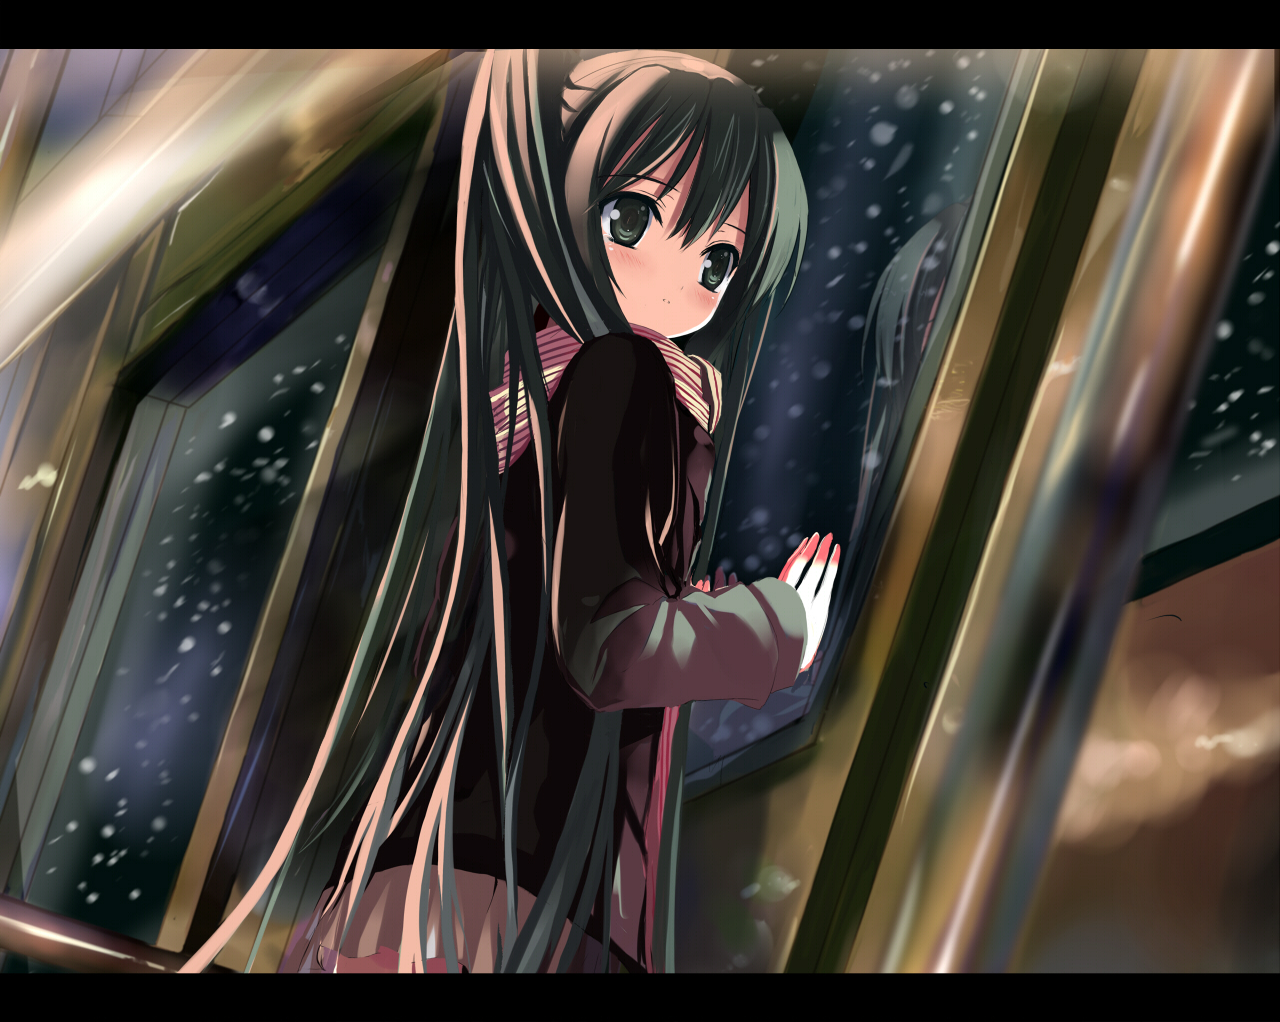
\includegraphics[scale=0.5]{2583887_p0.jpg}\end{center}
\newpage
